%\documentclass[aspectratio=169]{beamer}
\documentclass{beamer}
\usepackage[utf8x]{inputenc}
%\usepackage{default}
\usepackage{verbatim}
\usepackage{graphicx}
\usepackage{transparent}
\usepackage{listings}
\usepackage{qtree}

\title{Plucking Pictures from Publications}
\subtitle{I don't know what I'm doing!}
\author{Maarten Inja \and Maarten de Waard}
\institute[UvA]{University of Amsterdam}
\date[2014]{Intelligent Systems Project, June 26, 2014}
\logo{
\includegraphics[width=45px]{resources/uva}}
\usetheme{Berkeley}
\usecolortheme{sidebartab}
\usefonttheme{structuresmallcapsserif}
\newcommand{\slide}[2]
{
\begin{frame}
\frametitle{#1} 

#2

\end{frame}
}

\begin{document}

% \usebackgroundtemplate{
% {\transparent{0.5}\includegraphics[width=\paperwidth, % height=\paperheight]{resources/dna}}
% }
\begin{frame}
\titlepage
\end{frame}

\slide{Table of Contents}
{
	\tableofcontents
}

\section{Introduction}
\slide{Image Segmentation}
{
% We want to introduce the problem:
%	- Tell about image segmentation
%		Segment image into several classes..?
	What do we want to tell about image segmentation?
}
\subsection{Dataset}
\slide{Dataset - Overview}
{
	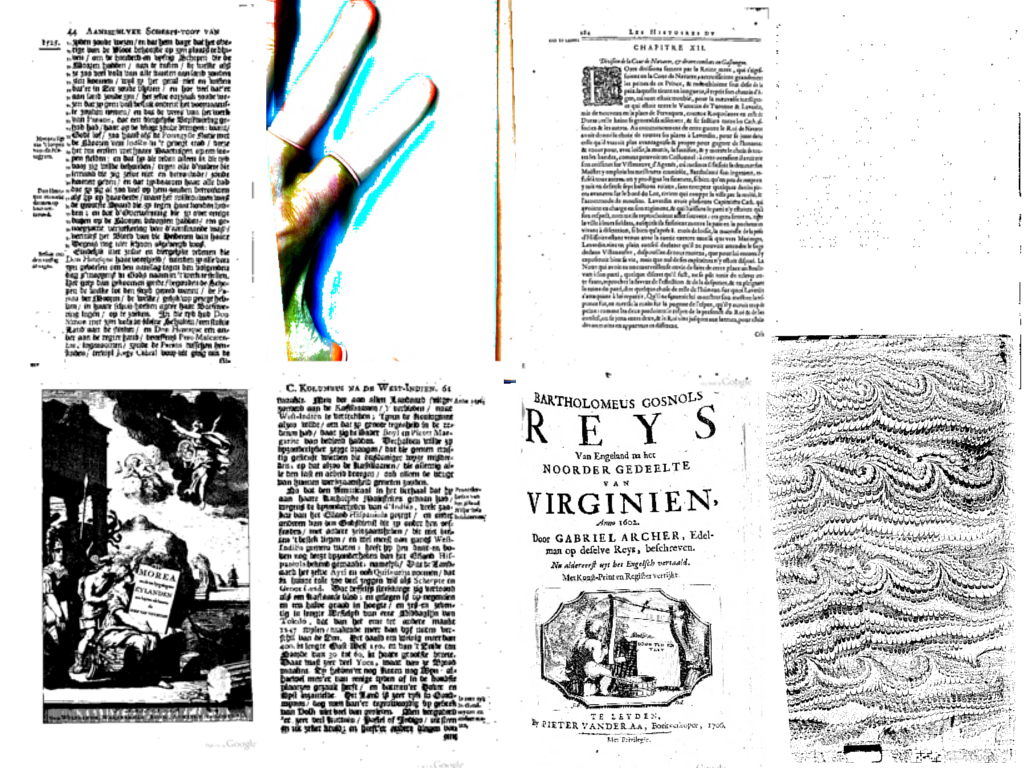
\includegraphics[width=.8\paperwidth]{resources/example1}
}
\slide{Dataset - Problem}
{
	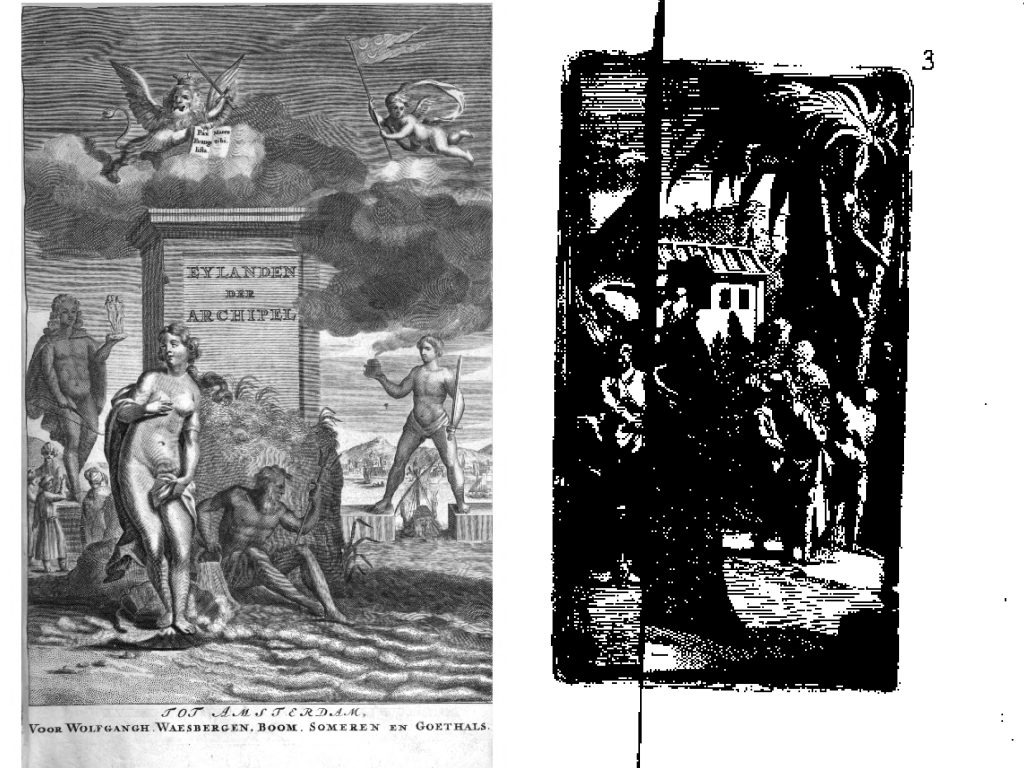
\includegraphics[width=.8\paperwidth]{resources/example2}
}

\section{Methods}
% Briefly explain HOG features
\slide{Features}
{
	\begin{block}{Hog Features}
	Steps for computing Hog Features\cite{dalal2005histograms}:
	\begin{enumerate}
		\item Global image normalisation
		\item Compute the gradient images
		\item Compute gradient histograms in 8 directions
		\item Normalise across blocks
		\item Flatten into a feature vector
	\end{enumerate}
	\end{block}
}
\begin{frame}[allowframebreaks]{Hog Examples}
	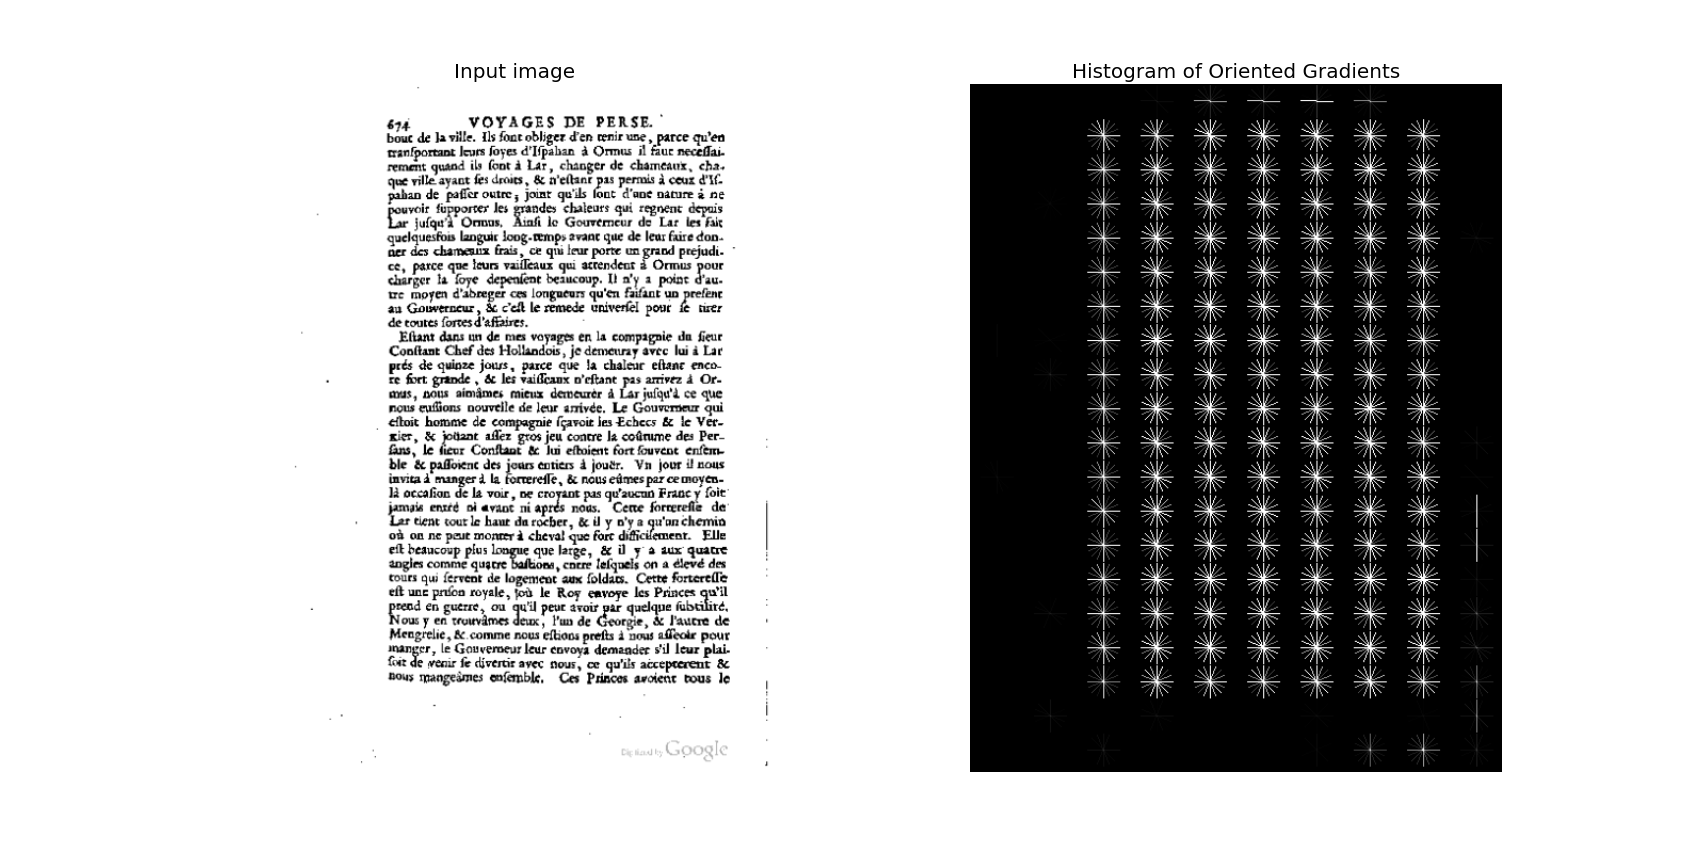
\includegraphics[trim=85px 0cm 0cm 0cm, clip=true, width=.8\paperwidth]{resources/text1}\\
\framebreak
	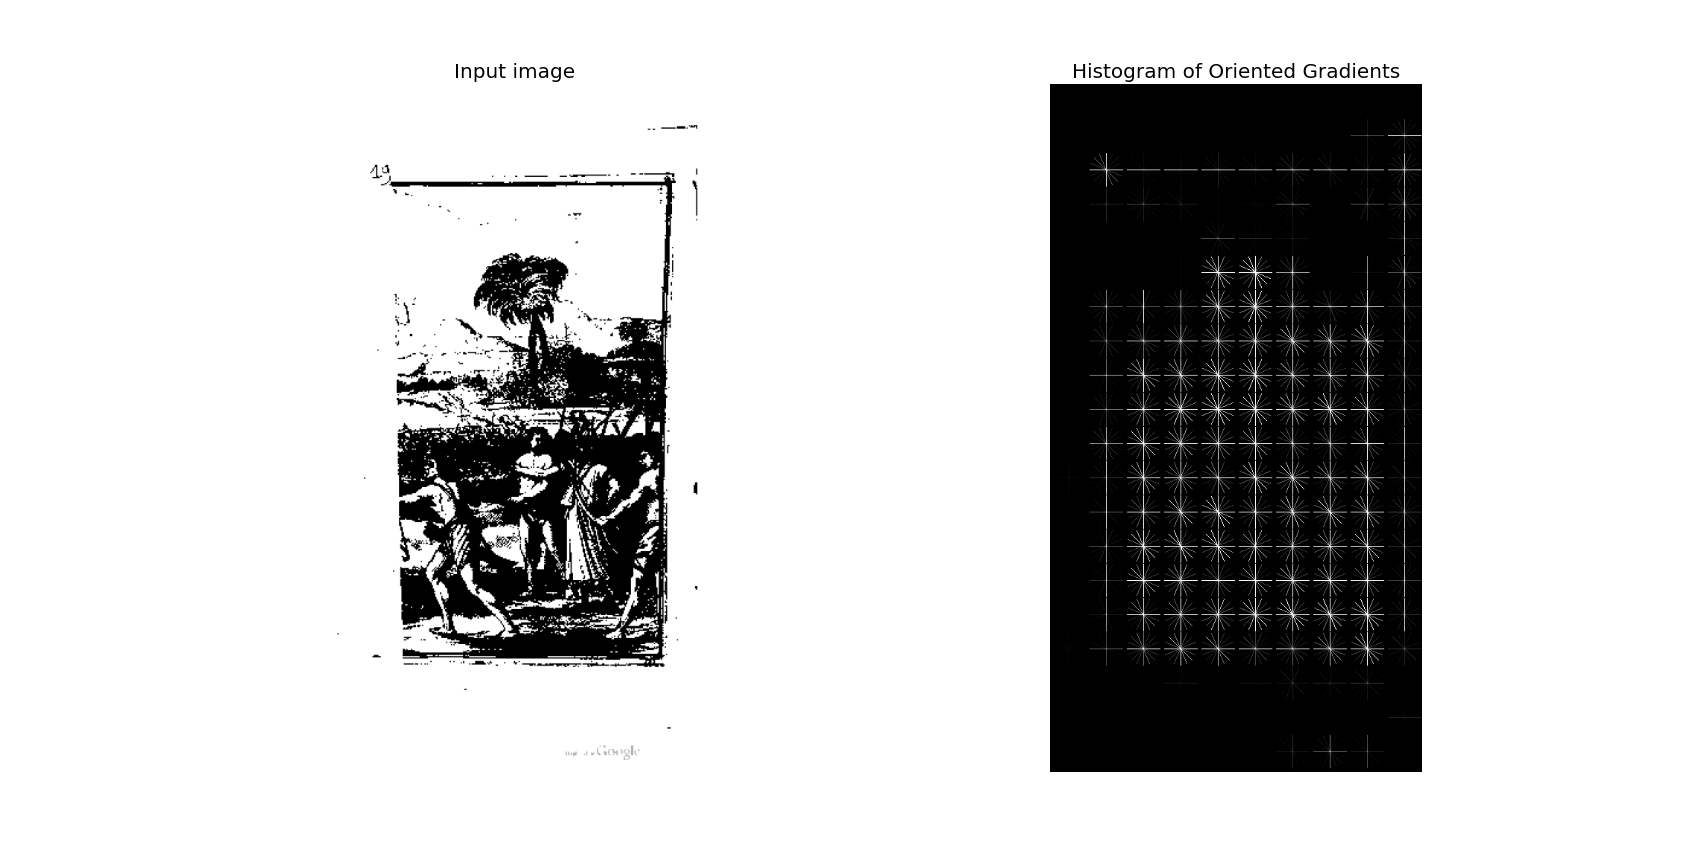
\includegraphics[width=.8\paperwidth]{resources/image1}\\
\framebreak
	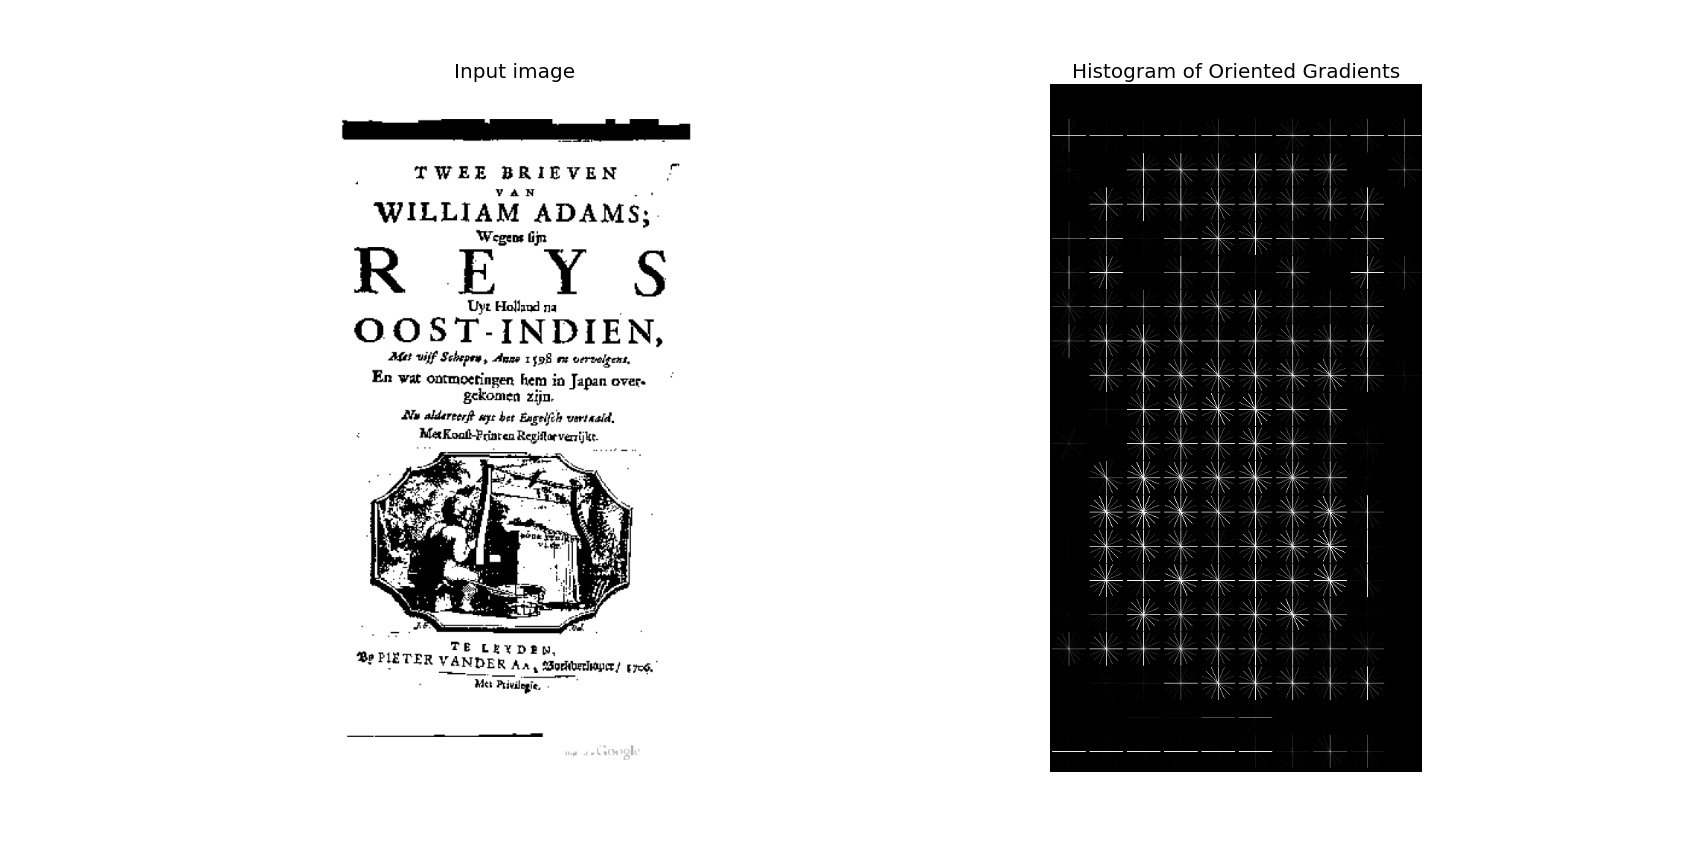
\includegraphics[width=.8\paperwidth]{resources/text_and_image1}
\end{frame}


\subsection{Classification}
% Explain SVM i.c.w. HOG features for pages

\subsection{Localization}
% Explain CRF and SSVM

\section{Results}
% Show results for classification
% Show results for different usages of SSVM

\section{Demo}
% Show which images are found (and which are not?) in a live demo

\section{Future Work}
% Improvements: 
% - Different kinds of features
% - 

\section{}

\slide{Questions and Discussion}
{}
\begin{frame}[allowframebreaks]
        \frametitle{References}
        \bibliographystyle{amsalpha}
        \bibliography{references.bib}
\end{frame}
\end{document}
